\chapter{User interface design}
\label{ch:ui_design}
As already stated earlier, we have different interfaces for the mobile
application and the web application.
The main idea is to initially establish a common design language (colors,
fonts, look of reusable components) which can then be applied to both
interfaces. In this regard we have provided some early mockups of the main pages
of both interfaces in the RASD (subsection 3.1.1 -- User interfaces).

Here we give a better detail of the flow of the application, also including
some pages of minor importance that were not shown in the RASD.
In the following diagrams the boxes represent the different pages and the
arrows the transitions from a page to another. The arrow labels indicate the
conditions(s) which trigger a particular transition.

\begin{figure}[ht]
    \centering
    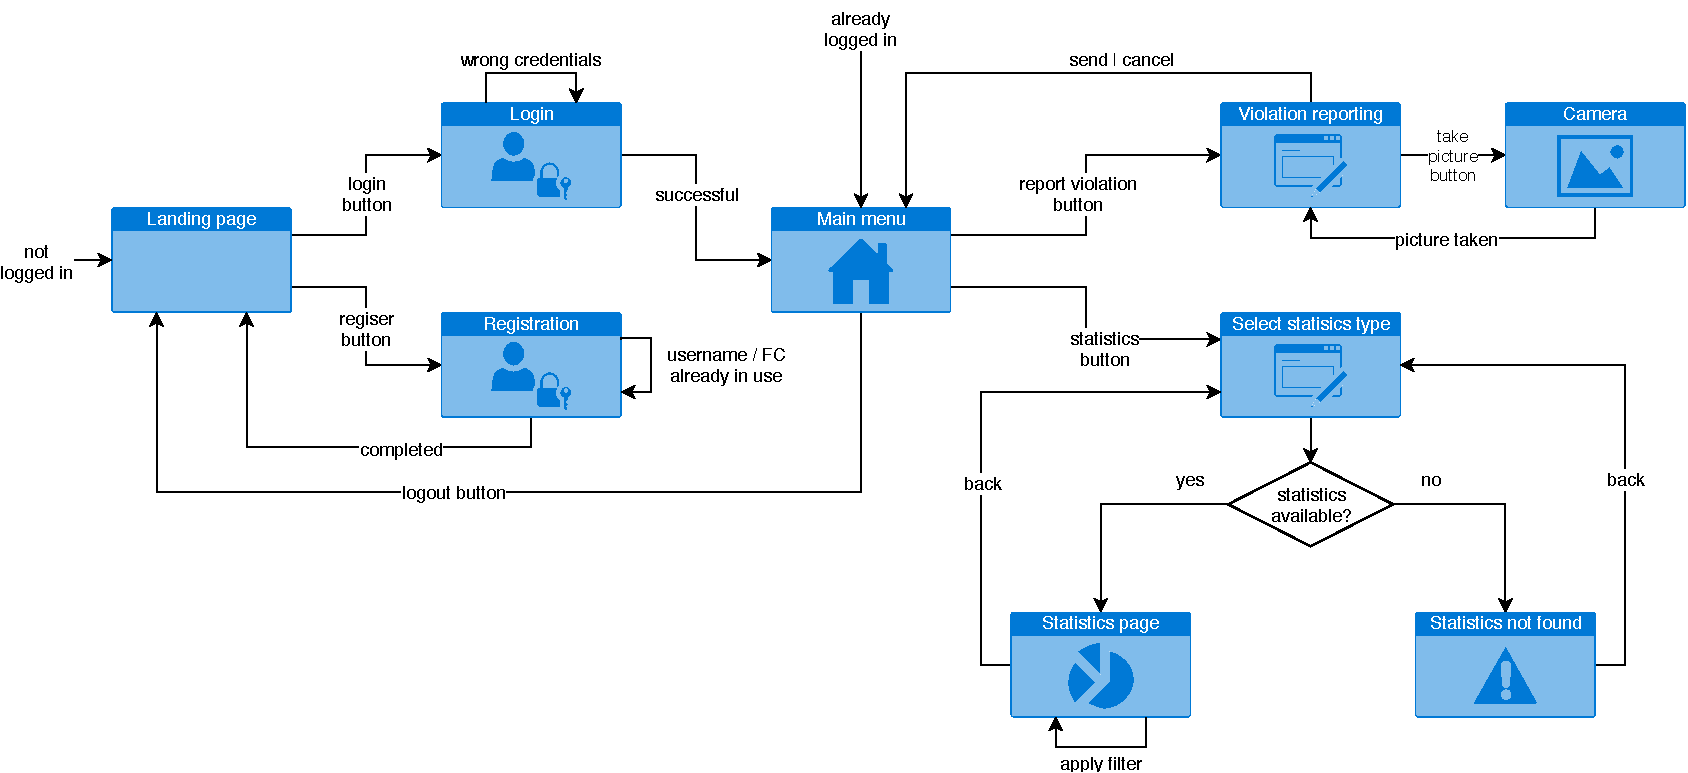
\includegraphics[width=\textwidth]{dd_ux_mobile}
    \caption{UX diagram for the mobile app}
    \label{fig:ux_mobile}
\end{figure}

Figure \vref{fig:ux_mobile} shows the UX diagram for the mobile application.
When the user opens the application on his smartphone, the first check is
whether he is already logged in or not. If he's not, the \emph{landing page}
will be shown, which enables him to login or register, otherwise the user
is directly taken to the \emph{main menu}.
Once in the \emph{main menu} the user can decide whether to report a violation,
view statistics or log out (this was not shown in the previous mockups).
For conciseness the links to come back from this page are not shown in the
diagram.

In case the user decides to report a violation, he will be taken to the
\emph{violation reporting page}, which is essentially a form that also
requires to take a photo. The process of reporting a violation has been already
described in the use cases.

In case the user decides to view statistics, he will be first presented
with a set of possible types of statistics (e.g.\ by month, by type).
He will select one of these types and the system will try to compute those
statistics. In case they are not available (e.g.\ there is no sufficient data
for violations in the surrounding area), then the user is brought to an
\emph{error page} from which he can go back and try with another type.
If everything goes right, instead, the user is brought to the
\emph{statistics page}; note that here the rendering of the statistics
(histogram, map, list) depends on the selected type. From here the user
can apply additional filters (restrict to a specific area, time period
or violation type).

\begin{figure}[ht]
    \centering
    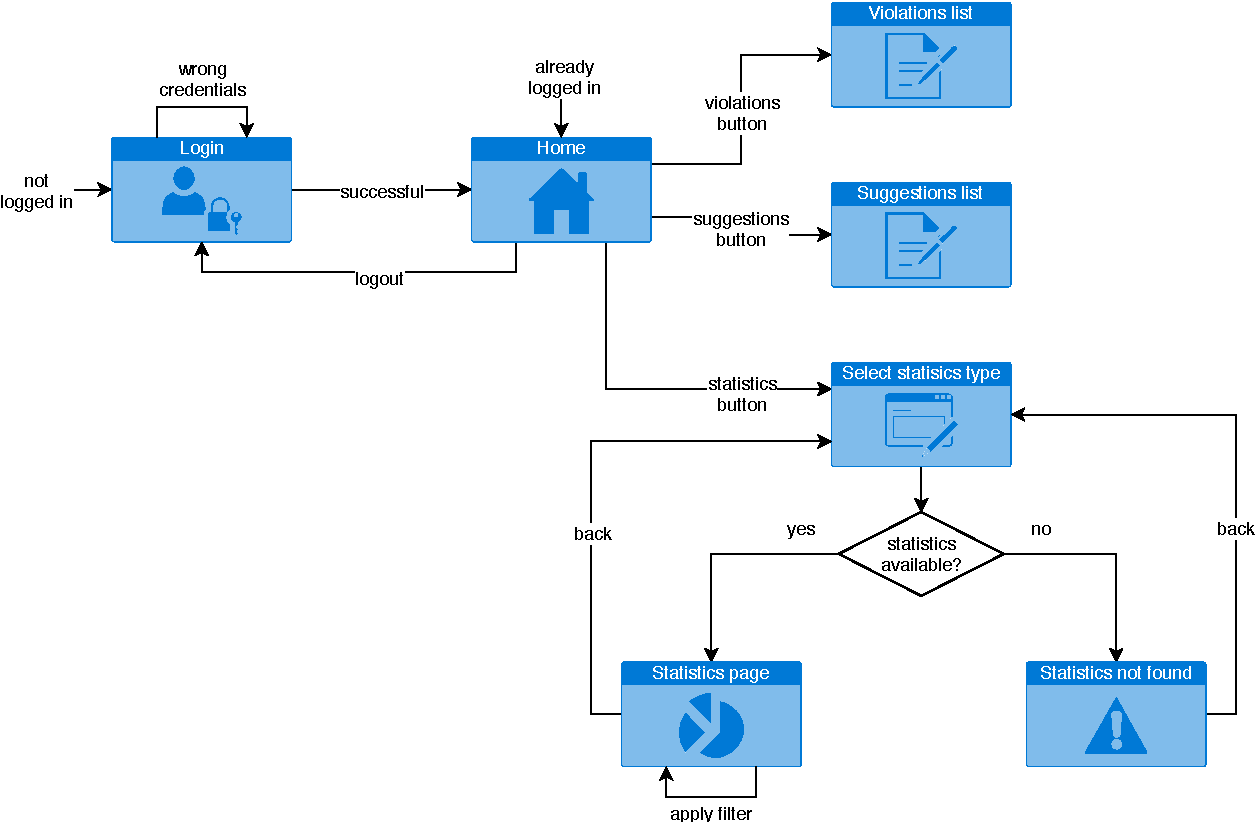
\includegraphics[width=\textwidth]{dd_ux_web}
    \caption{UX diagram for the web app}
    \label{fig:ux_web}
\end{figure}

Figure \vref{fig:ux_web} shows the UX diagram for the web application.
When the operator navigates to the website he will be presented with a
\emph{login page} if he's not already logged in, otherwise he will be
taken directly to the \emph{main menu}.
From the \emph{main menu} the operator can access the main functionalities
of the system, and he can also decide to \emph{log out}.

In case he clicks on the violations button, he will be taken to the
\emph{violations list} page, which shows all the most recently reported
violations that belong to that specific authority; violations that are still
pending for approval are shown at the top.
From here the operator can click on the \emph{info button} of a violation:
this will expand the list item to a card that shows the details of a the report.
If the violation is still unrevised, this card will also contain an two action
buttons to accept or discard the violation, respectively.
The list of violations can be implemented as an \emph{infinite scrolling list}:
initially only the most recent $N$ violations are retrieved, enough to fill
the page; then as the operator scrolls down the next $N$ violations are
retrieved from the server, and so on.

The suggestions button is only shown if the \emph{SmartSuggestions}
functionality is active for the current municipality. If the operator clicks on
it he's taken to the \emph{suggestions list} page.
This is very similar to the previous one, because it involves viewing a list
of suggestions, some of which are new and can be expanded to be marked as
\emph{carried out}. Also here we can apply the technique of the
\emph{infinite scrolling list}.

If the operator clicks on the statistics button, the process is pretty much the
same of the mobile application, detailed before.
The only things to keep in mind are that the authority also has the possibility
to see the licence plate numbers associated to violations.
Here, since this page will primarily viewed on the large screen of a PC,
we can show more data in a single page than in the mobile application
(as suggested by the mockups).

As an additional consideration, since the website can be viewed from devices
(smartphone, tablets, laptops, desktop PCs), its interface can be made
\emph{responsive} to adapt to the various screen sizes. At least this should be
done for the \emph{violations list} page, which can be useful for field
operators.